\chapter{\label{capterParabolicOptimalControlProblems}Parabolic optimal control problems}

\section{Introduction to the problem}
Our optimization problem is based on the problem that is presented in \cite{doi:10.1137/070694016}. We consider a state variable $u$ and a control variable $q$, defined on $(0,T)\times\Omega$ with $T\in\mathbb{R}$ and $\Omega\subset\mathbb{R}^n$.

The goal of this thesis is to minimize the function
\begin{subequations}
\label{conProb}
\begin{gather}
J(q,u)=\frac{1}{2}\int_0^T\int_\Omega(u(t,x)-\hat{u}(t,x))^2\,\mathrm{d}x\,\mathrm{d}t+\frac{\alpha}{2}\int_0^T\int_\Omega q(t,x)^2\,\mathrm{d}x\,\mathrm{d}t\label{objFun},\\
%\end{equation}
\intertext{subject to the constraints}
%\begin{equation}
\begin{aligned}
	\partial_tu-\Delta u&=f+q&\text{ in }(0,T)\times\Omega,\\
	u(0)&=u_0&\text{ in }\Omega,
\end{aligned}
\label{constraints}
\end{gather}
\end{subequations}
with homogeneous Dirichlet boundary conditions on $(0,T)\times\partial\Omega$.

Let $V=H_0^1(\Omega)$, $H=L^2(\Omega)$ and $I=(0,T)$. We define our state space as
\begin{displaymath}
X:=\{v\mid v\in L^2(I,V)\text{ and }\partial_tv\in L^2(I,V^*)\}
\end{displaymath}
and the control space as
\begin{displaymath}
Q:=L^2(I,L^2(\Omega)).
\end{displaymath}
The notion of the inner products and norms on $L^2(\Omega)$ and $L^2(I,L^2(\Omega))$ is introduced as
\begin{align*}
(v,w)&:=(v,w)_{L^2(\Omega)},&(v,w)_I&:=(v,w)_{L^2(I,L^2(\Omega))},\\
\|v\|&:=\|v\|_{L^2(\Omega)},&\|v\|_I&:=\|v\|_{L^2(I,L^2(\Omega))}.
\end{align*}
By using the inner product, the weak form of the state equations \eqref{constraints} for $q,f\in Q$ and $u_0\in V$ is given as
\begin{equation}
\label{weakEq}
\begin{aligned}
	(\partial_tu,\phi)_I+(\nabla u,\nabla\phi)_I&=(f+q,\phi)_I&\forall\phi\in X,\\
	u(0)&=u_0&\text{ in }\Omega.
\end{aligned}
\end{equation}
With the weak state equations \eqref{weakEq}, we define the weak formulation of the optimal control problem \eqref{conProb} as
\begin{equation}
\label{weakProb}
\text{Minimize }J(q,u):=\frac{1}{2}\|u-\hat{u}\|_I^2+\frac{\alpha}{2}\|q\|_I^2\text{ subject to \eqref{weakEq} and }(q,u)\in Q\times X.
\end{equation}

Now we cite two results of the problems \eqref{weakEq} and \eqref{weakProb}.

\begin{prop}[\cite{doi:10.1137/070694016}]
\label{uniqueU}
For fixed $q,f\in Q$, and $u_0\in V$ there exists a unique solution $u\in X$ of problem \eqref{weakEq}. Moreover, the solution exhibits the improved regularity
\begin{displaymath}
u\in L^2(I,H^2(\Omega)\cap V)\cap H^1(I,L^2(\Omega))\hookrightarrow C(\bar{I},V).
\end{displaymath}
It holds the stability estimate
\begin{displaymath}
\|\partial_tu\|_I+\|\nabla^2u\|_I\leq C\{\|f+q\|_I+\|\nabla u_0\|\}.
\end{displaymath}
\end{prop}

%evtl rauslassen
\begin{prop}[\cite{doi:10.1137/070694016}]
For given $f,\hat{u}\in L^2(I,H)$, $u_0\in V$, and $\alpha>0$, the optimal control Problem \eqref{weakProb} admits a unique solution $(\bar{q},\bar{u})\in Q\times X$. The optimal control $\bar{q}$ posesses the regularity
\begin{displaymath}
\bar{q}\in L^2(I,H^2(\Omega))\cap H^1(I,L^2(\Omega)).
\end{displaymath}
\end{prop}

Due to the existence and uniqueness results from Proposition \ref{uniqueU}, we define $u(q)$ as the unique solution of \eqref{weakEq} with respect to some $q\in Q$. This enables us to define a reduced cost functional $j:Q\to \mathbb{R}$ that is only dependent on the control $q$ as
\begin{displaymath}
j(q):=J(q,u(q)).
\end{displaymath}
From now on, the optimal control problem that we examine is:
\begin{equation}
\label{redProb}
\text{minimize }j(q)\text{ subject to }q\in Q.
\end{equation}

\section{Finite element discretization}
In order to solve the optimization problem \eqref{redProb} numerically, the discretization of our model is now discussed. We begin with the presentation of the discretization in space with a n-D continuous Galerkin method. Then, we look at the discretization in time, which is done with a 1D continuous Galerkin method. From now on, we will also discuss some implementation details, so, in this chapter, how we handle the calculation of the objective function $j$. To solve the partial equations of \eqref{weakEq}, we use the Python package pyMOR.

\subsection{\label{SubsectionDiscretizationInSpace}Discretization in space}
The discretization in space is shown on a 2-dimensional rectangular space $\Omega\subset\mathbb{R}^2$ with linear finite elements. We assume to have a vertex set $\mathcal{V}=(x_1,\dotsc,x_N)\in(\mathbb{R}^2)^N$ with a convex hull that is equal  to $\bar{\Omega}$ and $x_i\neq x_j$ for all $i\neq j$ in $\{1,\dotsc,N\}$. Let $\hat{T}=\{(x,y)\in[0,1]^2\mid y \leq 1-x\}$ be the reference triangle. Then,
\begin{displaymath}
\theta_l(\xi)=x_{l_1} + D\theta_l \begin{pmatrix} \xi_1 \\ \xi_2 \end{pmatrix} \text{ with } D\theta_l = \begin{pmatrix} x_{l_2}-x_{l_1} & x_{l_3}-x_{l_1} \end{pmatrix}
\end{displaymath}
is a transformation from the reference triangle $\hat{T}$ to some other triangle $T_l$ with the corners $x_{l_1}, x_{l_2}, x_{l_3}\in\mathcal{V}$.

We define now a mesh $\mathcal{T}=\{T_l\}$ which consists of triangles $T_l=\theta_l(\hat{T})$, where $T_l\cap T_m$ for $T_l,T_m\in\mathcal{T}$ is either a common side, a common corner, or empty, and where $\bar{\Omega}=\cup_{T_l\in\mathcal{T}}T_l$. We also assume that every vertex in $\mathcal{V}$ is a corner of at least one triangle of $\mathcal{T}$.

In our implementation, we discretize a rectangular domain by specifying the number of grid intervals first. Then, we divide the domain into smaller rectangles of the same size, so that the number of rectangles along the $x$- and the $y$-axis is equal to the predefined number of grid intervals. Each smaller rectangular unit is then divided into four equally sized triangles by adding a vertex into the center of the rectangle which is connected with the corners of the unit. The vertex set of the whole domain is now given by the union of the corners of all triangles. As an example, if we have given a domain $\Omega = [a, a]$ with $a>0$ and we define the number of grid intervals as $2$, then our mesh would look like that:
\begin{figure}
    \centering
    %\textbf{Your title}\par\medskip
    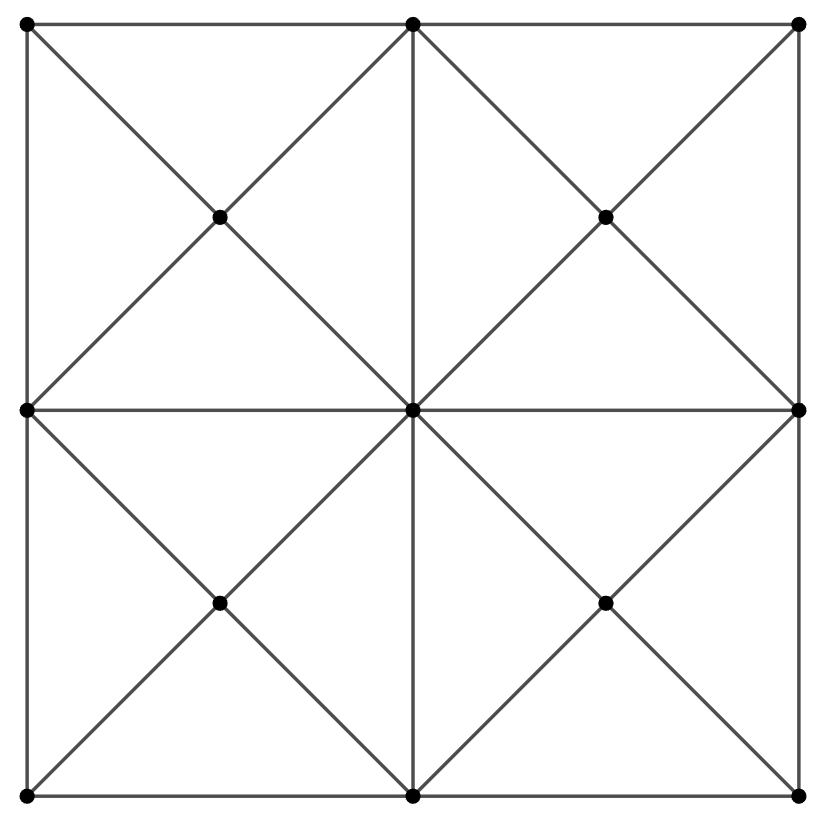
\includegraphics[height=8cm]{mesh.png} 
    \caption{Example of a mesh with $2$ grid intervals in a square-shaped domain.}
\end{figure}
%\begin{center}
%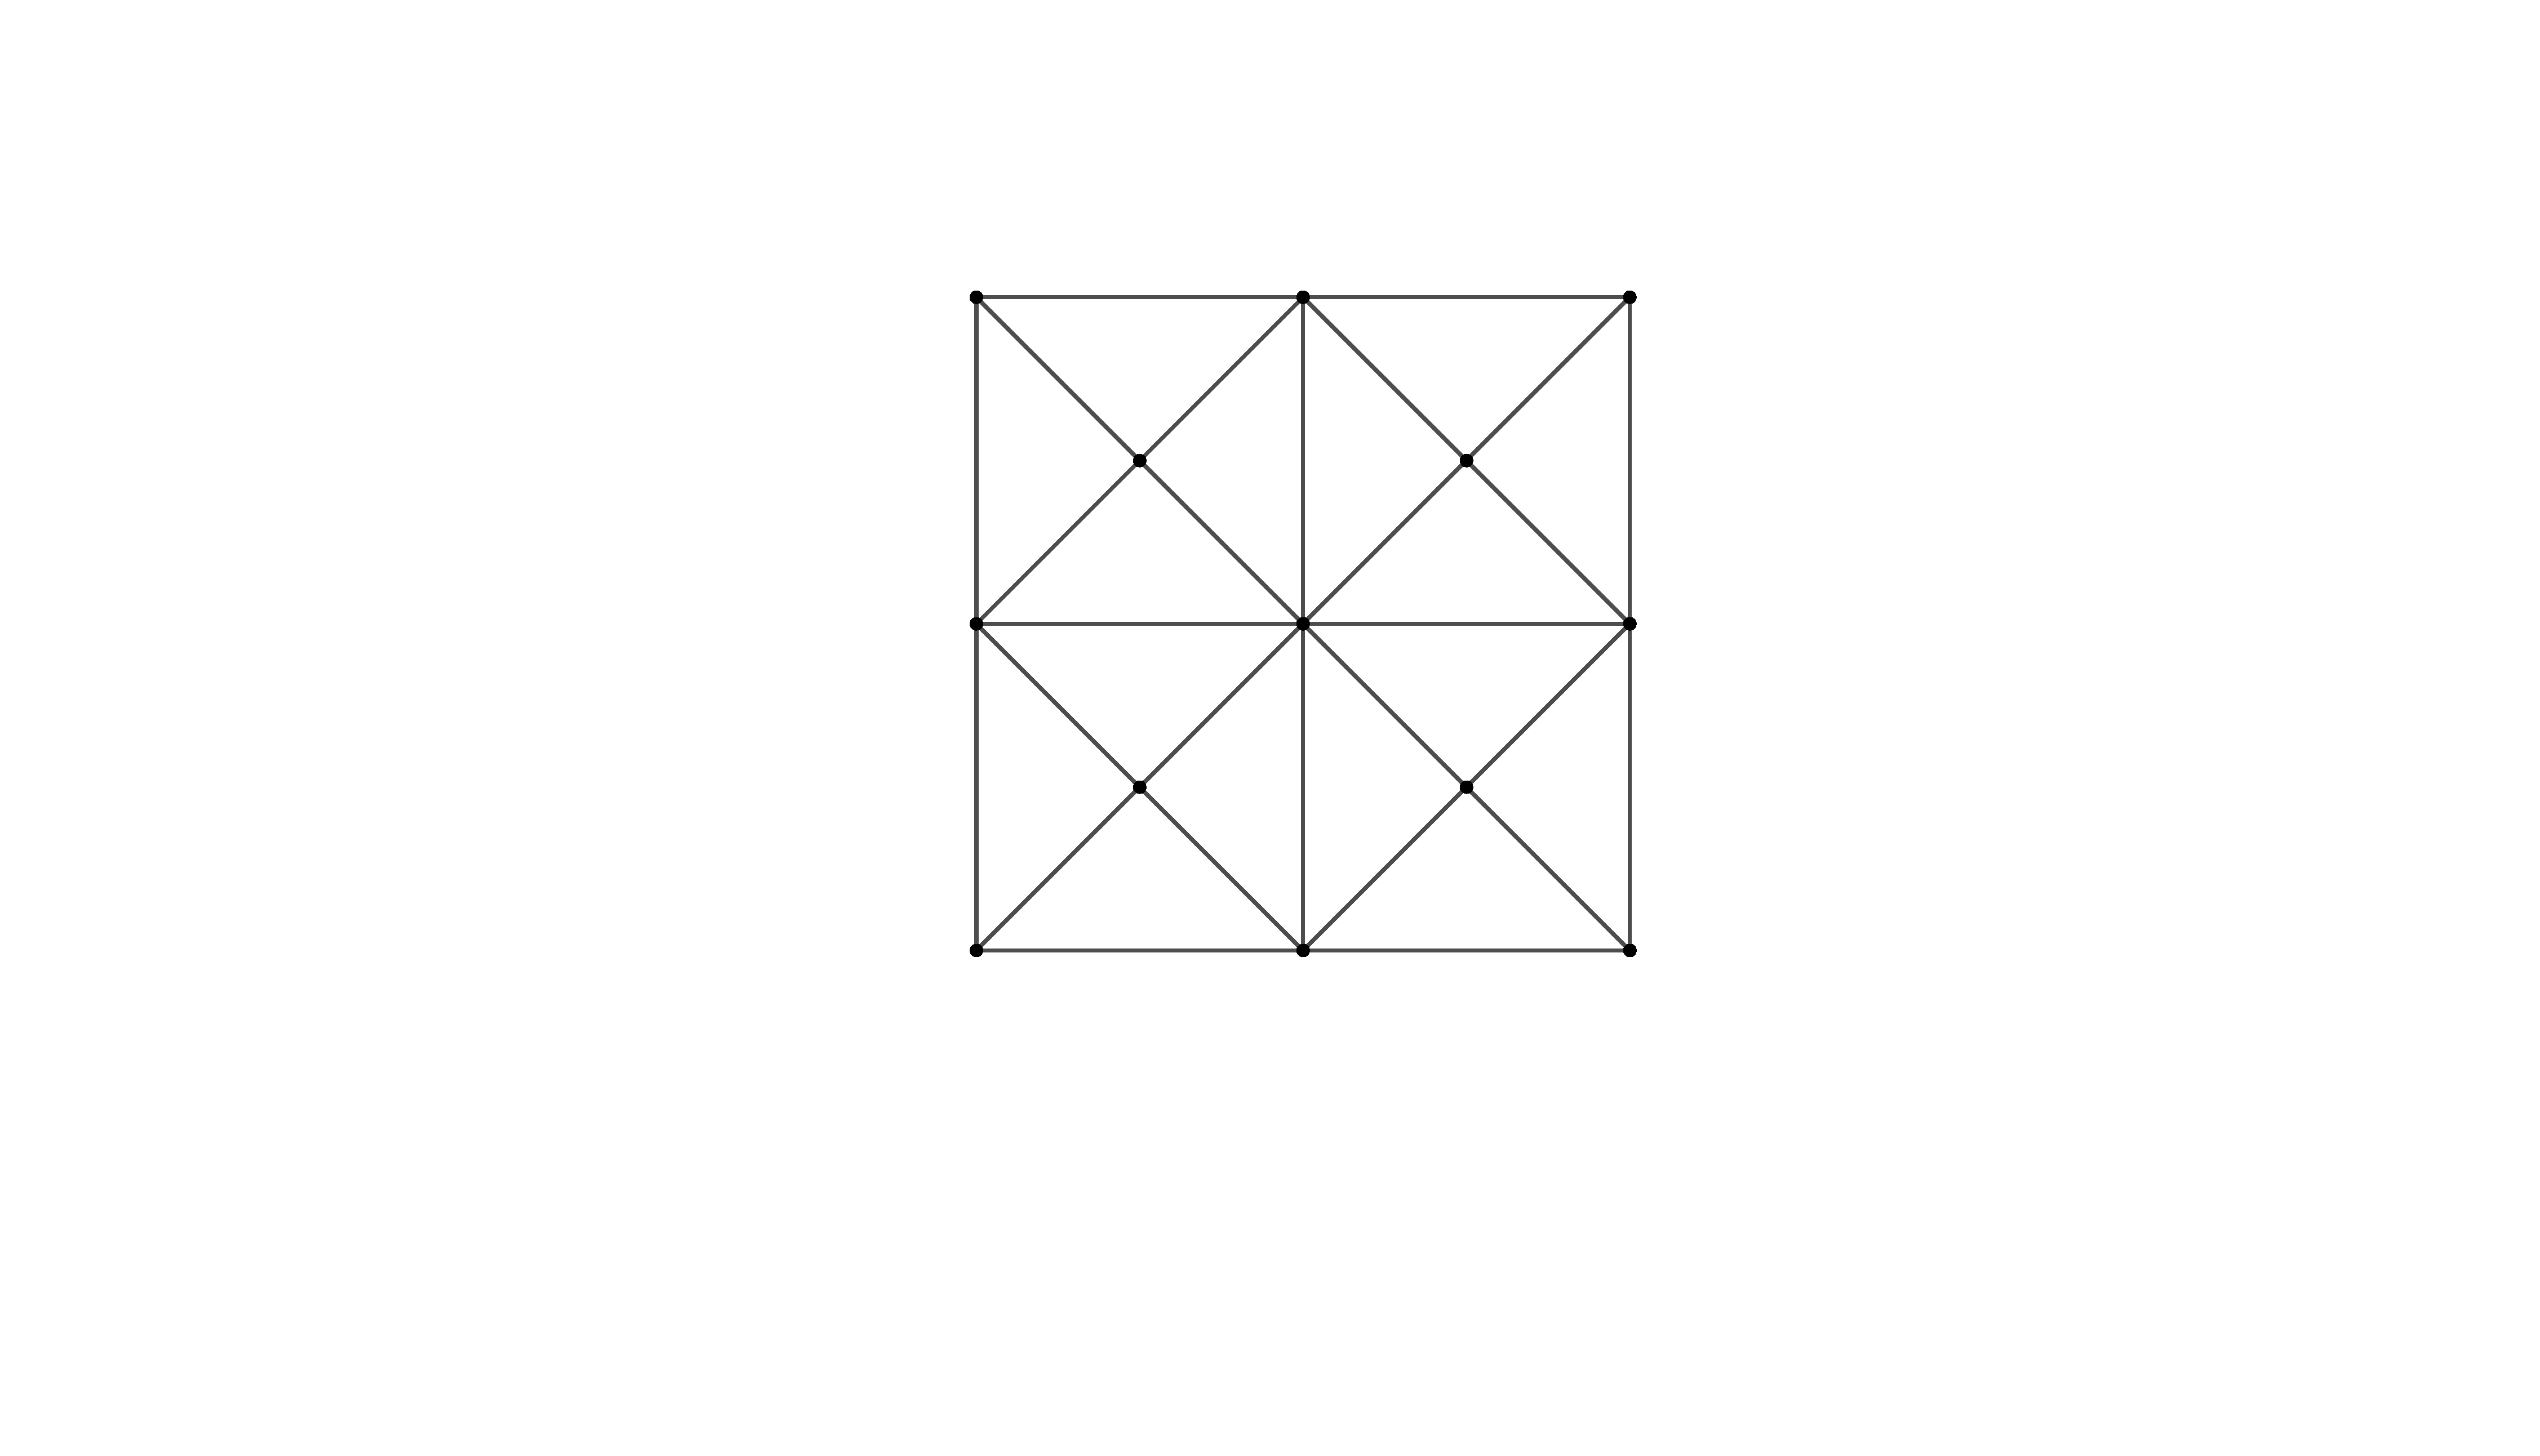
\includegraphics[height=8cm]{discretization.pdf} 
%Example of a mesh with $2$ grid intervals in a cuboid domain.
%\end{center}

Now, let $\mathcal{P}_1(\hat{T}, \mathbb{R})$ be the space of polynomials up to order 1 in $\hat{T}$. Then, $\{\psi_1, \psi_2, \psi_3\}$ with $\psi_1(\xi)=1-\xi_1-\xi_2, \psi_2(\xi)=\xi_1, \psi_3(\xi)=\xi_2$ defines a basis of $\mathcal{P}_1(\hat{T}, \mathbb{R})$.
%Therefore, $\{\phi_1, \phi_2, \phi_3\}$ with $\phi_{l_m}= \psi_m \circ \theta_l^{-1}$ for $m=1, 2, 3$ defines a basis of $\mathcal{P}_1(T, \mathbb{R})$.
Using this basis, we set
\begin{displaymath}
%V_h=\{v\in C(\Omega)\mid  v|_{T_l}\in\operatorname*{span}\{\phi_{l_1}, \phi_{l_2}, \phi_{l_3}\}\forall T_l\in\mathcal{T}\}
V_h=\operatorname*{span}\{\phi_i, i=0,\dotsc,N\}\cap V
\end{displaymath}
as the finite element space of our state variables with
\begin{displaymath}
\phi_i|_{T_l}=\begin{cases}
0 & \text{ if $x_i\notin T_l$}\\
\psi_1 \circ \theta_l^{-1} & \text{ if $\theta_l\left(\begin{pmatrix} 0 \\ 0 \end{pmatrix}\right)=x_i$}\\
\psi_2 \circ \theta_l^{-1} & \text{ if $\theta_l\left(\begin{pmatrix} 1 \\ 0 \end{pmatrix}\right)=x_i$}\\
\psi_3 \circ \theta_l^{-1} & \text{ if $\theta_l\left(\begin{pmatrix} 0 \\ 1 \end{pmatrix}\right)=x_i$}
\end{cases} 
\end{displaymath}
for all $T_l\in\mathcal{T}$ and $i=1,\dotsc,N$.

By construction, every $u\in V_h$ is uniquely defined by
\begin{displaymath}
u=\sum_{i=1}^NU_i\phi_i
\end{displaymath}
with $U_i=u(x_i)$.\\

Now we want to calculate $\int_\Omega u \cdot v \,\mathrm{d}x$ and $\int_\Omega \nabla u \cdot \nabla v \,\mathrm{d}x$ for all $u,v\in  V_h$. In order to do that, we set the mass matrix $M_n = \left(\int_\Omega \phi_i \cdot \phi_j \,\mathrm{d}x\right)_{i,j=1,\dotsc,N}$ and the stiffness matrix $L_n = \left(\int_\Omega \nabla\phi_i \cdot \nabla\phi_j \,\mathrm{d}x\right)_{i,j=1,\dotsc,N}$. Let%We calculate these integrals by taking the sum of the integrals over all triangles $T_l\in\mathcal{T}$ where $\phi_i$ and $\phi_j$ are not zero, so all triangles $T_l$ with $x_i,x_j\in T_l$
\begin{displaymath}
U=\begin{pmatrix} U_1 \\ \vdots \\ U_n \end{pmatrix}\text{ and }V=\begin{pmatrix} V_1 \\ \vdots \\ V_n \end{pmatrix}.
\end{displaymath}
Then we have
\begin{displaymath}
\int_\Omega u \cdot v \,\mathrm{d}x=U^TM_nV\text{ and }\int_\Omega \nabla v \cdot \nabla u \,\mathrm{d}x=U^TL_nV.
\end{displaymath}


\subsection{\label{SubsectionDiscretizationInTime}Discretization in time}
At first, we partition the time interval $\bar{I}=[0,T]$ as
\begin{displaymath}
\bar{I}=\{0\}\cup I_1\cup I_2\cup\dotsb\cup I_M
\end{displaymath}
with subintervals $I_m=(t_{m-1},t_m]$, where $t_m=m\frac{T}{M}$ for $m=0,\dotsc, M$ and $M\in\mathbb{N}$. We want that the discretizations of our functions are continuous in $\bar{I}$ and piecewise polynomial of order 1 in all subintervals $I_m$, so the discretization space of our state variables is
\begin{displaymath}
X_{k,h}:=\{v\in C(\bar{I},V_h)\mid v |_{I_m}\in\mathcal{P}_1(I_m,V_h),m=1,2,\dotsc,M\},
\end{displaymath}
where $\mathcal{P}_1(I_m,V_h)$ denotes the space of polynomials up to order 1, defined on $I_m$ with values in $V_h$.
Similarly, we define the time-discretized space of our control variables as
\begin{displaymath}
Q_d:=\{v\in C(\bar{I},H)\mid v |_{I_m}\in\mathcal{P}_1(I_m,H),m=1,2,\dotsc,M\}\supset X_{k,h}.
\end{displaymath}

By using the Lagrange basis of $\mathcal{P}_1(I_m,\mathbb{R})$, we can write every function $v \in Q_d$ as
\begin{displaymath}
v(t,\cdot)=\left(m-t\frac{M}{T}\right) v_{m-1}(\cdot)+\left(t\frac{M}{T}-m+1\right) v_m(\cdot)\text{ for }t\in I_m,
\end{displaymath}
where $v_m(\cdot)=v(t_m,\cdot)$.


\subsection{Crank-Nicolson scheme}
Now, we solve the weak state equations \eqref{weakEq} for the state $u\in X_{k,h}$, the control $q\in Q_d$, and $f\in Q$ numerically. For $m=0$, we set
\begin{displaymath}
U_0=\begin{pmatrix} U_{0,1} \\ \vdots \\ U_{0,n} \end{pmatrix},
\end{displaymath}
where $U_{0,i}=u_0(x_i)$ for $i=1,\dotsc,N$.

For $m=1,\dotsc,M$, we get with the Crank-Nicolson scheme that for all $v\in V_h$:
\begin{eqnarray*}
(u_m,v) + \frac{T}{2M}(\nabla u_m, \nabla v) & = &(u_{m-1},v) - \frac{T}{2M}(\nabla u_{m-1}, \nabla v)\\
&& + \frac{T}{2M}(f_{m-1} + q_{m-1}, v) + \frac{T}{2M}(f_m + q_m, v),
\end{eqnarray*}
where $u_m$ is a time discretization of $u$ at the time step $t_m$, while $f_m=f(t_m, \cdot)$ and $q_m=q(t_m,\cdot)$. To solve the above equation, we define the matrix $\tilde{M}_n\in\mathbb{R}^{N\times N}$ as
\begin{displaymath}
\left(\tilde{M}_n\right)_{i,j}=\begin{cases}
0 & \text{ if $x_i$ or $x_j$ in $\partial\Omega$ and $i \neq j$}\\
1 & \text{ if $x_i$ or $x_j$ in $\partial\Omega$ and $i = j$}\\
\left(M_n\right)_{i,j} & \text{ else}
\end{cases}
\end{displaymath}
and the matrix $\tilde{L}_n\in\mathbb{R}^{N\times N}$ as
\begin{displaymath}
\left(\tilde{L}_n\right)_{i,j}=\begin{cases}
0 & \text{ if $x_j$ in $\partial\Omega$}\\
\left(L_n\right)_{i,j} & \text{ else,}
\end{cases}
\end{displaymath}
so that $(u_m,v)=U_m^T\tilde{M}_nV$ and $(\nabla u_m,\nabla v)=U_m^T\tilde{L}_nV$ for all $m=0,\dotsc,M$, which is giving us
\begin{eqnarray*}
V^T\tilde{M}_n^TU_m + \frac{T}{2M} V^T\tilde{L}_n^T U_m &=& V^T\tilde{M}_n^TU_{m-1} - \frac{T}{2M} V^T\tilde{L}_n^T U_{m-1}\\
&&  + \frac{T}{2M}(f_{m-1} + q_{m-1}, v) + \frac{T}{2M}(f_m + q_m, v).
\end{eqnarray*}
In the pyMOR implementation, vectors $F_m$ for $m=0,\dotsc,M$ are defined such that $V^TF_m\approx(f_m + q_m, v)$ for all $v\in V_h$ and $\left(F_m\right)_i=0$ if the $i$-th entry in the vertex set $\mathcal{V}$ lies on the boundary of $\Omega$. By using these vectors, we get the equation
\begin{equation}
\label{crank_nicolson}
\left(\tilde{M}_n^T + \frac{T}{2M} \tilde{L}_n^T\right) U_m = \tilde{M}_n^TU_{m-1} - \frac{T}{2M} \tilde{L}_n^T U_{m-1} + \frac{T}{2M} F_{m-1} + \frac{T}{2M} F_m,
\end{equation}
which is solved after $U_m$ with functions from the Python package SciPy.

\subsection{\label{subsectionCalculationOfTheObjectiveFunctionValue}Calculation of the objective function value}
For fixed $\hat{u},f\in Q$, we define $u=u(q)$ for all $q\in Q_d$, so that it satisfies \eqref{crank_nicolson}. We calculate $j(q)$ now in the following way:
\begin{eqnarray*}
j(q) \approx& \frac{1}{2}\sum_{m=1}^M\int_{t_{m-1}}^{t_m}&\bigg(\left(m-t\frac{M}{T}\right) \left(u_{m-1}-\hat{u}_{m-1}\right)+\left(t\frac{M}{T}-m+1\right) \left(u_{m}-\hat{u}_{m}\right),\\
&&\left(m-t\frac{M}{T}\right) \left(u_{m-1}-\hat{u}_{m-1}\right)+\left(t\frac{M}{T}-m+1\right) \left(u_{m}-\hat{u}_{m}\right)\bigg)\,\mathrm{d}t\\
&+ \frac{\alpha}{2}\sum_{m=1}^M\int_{t_{m-1}}^{t_m}&\bigg(\left(m-t\frac{M}{T}\right) q_{m-1}+\left(t\frac{M}{T}-m+1\right) q_{m},\\
&&\left(m-t\frac{M}{T}\right) q_{m-1}+\left(t\frac{M}{T}-m+1\right) q_{m}\bigg)\,\mathrm{d}t.
\end{eqnarray*}
Integration by substitution yields
\begin{eqnarray*}
j(q) \approx& \frac{T}{6M}\sum_{m=1}^M&\left(u_{m-1}-\hat{u}_{m-1},u_{m-1}-\hat{u}_{m-1}\right) + \left(u_{m-1}-\hat{u}_{m-1},u_{m}-\hat{u}_{m}\right)\\
&&+ \left(u_{m}-\hat{u}_{m},u_{m}-\hat{u}_{m}\right)\\
&+ \frac{\alpha T}{6M}\sum_{m=1}^M&\left(q_{m-1},q_{m-1}\right) + \left(q_{m-1},q_{m}\right) + \left(q_{m},q_{m}\right)\\
\approx& \frac{T}{6M}\sum_{m=1}^M&\left(U_{m-1}-\hat{U}_{m-1}\right)M_n\left(U_{m-1}-\hat{U}_{m-1}\right)\\
&&+ \left(U_{m-1}-\hat{U}_{m-1}\right)M_n\left(U_{m}-\hat{U}_{m}\right)\\
&&+ \left(U_{m}-\hat{U}_{m}\right)M_n\left(U_{m}-\hat{U}_{m}\right)\\
&+ \frac{\alpha T}{6M}\sum_{m=1}^M&Q_{m-1}M_nQ_{m-1} + Q_{m-1}M_nQ_{m} + Q_{m}M_nQ_{m},
\end{eqnarray*}
where $\hat{U}_m=\left(\hat{u}(t_m, x_i)\right)_{i=1,\dotsc,N}$ and $Q_m=\left(q(t_m, x_i)\right)_{i=1,\dotsc,N}$ for $m=0,\dotsc,M$.

\section{Optimization of the control variable}

To optimize the control variable, we write every $q\in Q_d$, by using a fixed set of shape functions
\begin{equation}
\label{basisFuncionsList}
\Phi=\{\phi_1,\dotsc,\phi_{N_b}\}
\end{equation}
 with $\phi_1,\dotsc,\phi_{N_b}\in H$ and scalars $q_1^0,q_1^1,\dotsc,q_1^M,\dotsc,q_{N_b}^0,q_{N_b}^1\dotsc,q_{N_b}^M\in\mathbb{R}$, as
\begin{equation}
\label{discrContrVar}
q(t,x) = \sum_{i=1}^{N_b}\alpha_i(t)\phi_i(x)
\end{equation} 
with
\begin{displaymath}
\alpha_i(t)=\begin{cases}
q_i^{m-1}\left(m-t\frac{M}{T}\right) + q_i^m\left(t\frac{M}{T}-m+1\right) & \text{ if $t\in I_m$ with $m=1,\dotsc,M$}\\
q_i^0 & \text{ if $t=0$}
\end{cases}
\end{displaymath}
Each control variable that is written in this form can be represented as a vector
\begin{displaymath}
\mathbf{q}=\left[q_1^0,q_1^1,\dotsc,q_1^M,\dotsc,q_{N_b}^0,q_{N_b}^1\dotsc,q_{N_b}^M\right]^T\in\mathcal{D}:=\mathbb{R}^{N_q},
\end{displaymath} 
with $N_q = (M+1)\cdot N_b$. Therefore, we write
\begin{displaymath}
j(\mathbf{q}):=j(q)
\end{displaymath}
for each $q$ that is defined like in \eqref{discrContrVar}.

In the next chapters, we present algorithms that minimize $j(\mathbf{q})$ with respect to its control vector $\mathbf{q}$.
































































